\documentclass[10pt]{article}

\usepackage[margin=0.75in]{geometry}
\usepackage{amsmath, amssymb}
\usepackage{graphicx}
\usepackage[T1]{fontenc}
\usepackage{inconsolata}
\usepackage{titlesec}
\usepackage{fancyhdr}
\usepackage{microtype}

\graphicspath{{../}}

\setlength{\parindent}{0pt}
\setlength{\parskip}{4pt}
\renewcommand{\baselinestretch}{1.05}

\titleformat{\section}{\ttfamily\normalsize\bfseries\MakeUppercase}{\thesection}{0.6em}{}
\titlespacing*{\section}{0pt}{8pt}{2pt}
\titleformat{\subsection}{\ttfamily\small\MakeUppercase}{\thesubsection}{0.6em}{}
\titlespacing*{\subsection}{0pt}{6pt}{2pt}

\pagestyle{fancy}
\fancyhf{}
\renewcommand{\headrulewidth}{0pt}
\renewcommand{\footrulewidth}{0.5pt}
\fancyfoot[L]{\ttfamily\footnotesize 115-GILES-APPROXIMATE-SHEAR-WALL-QUANTITY}
\fancyfoot[C]{\ttfamily\footnotesize REV \today}
\fancyfoot[R]{\ttfamily\footnotesize \thepage}

\begin{document}

\noindent
\includegraphics[height=0.7cm]{logo}\hfill
{\ttfamily\normalsize\bfseries\MakeUppercase{115 Giles Approximate Shear Wall Quantity}}\quad
{\ttfamily\footnotesize\today}
\vspace{4pt}\hrule\vspace{6pt}

\section{Governing Lateral Load}

\noindent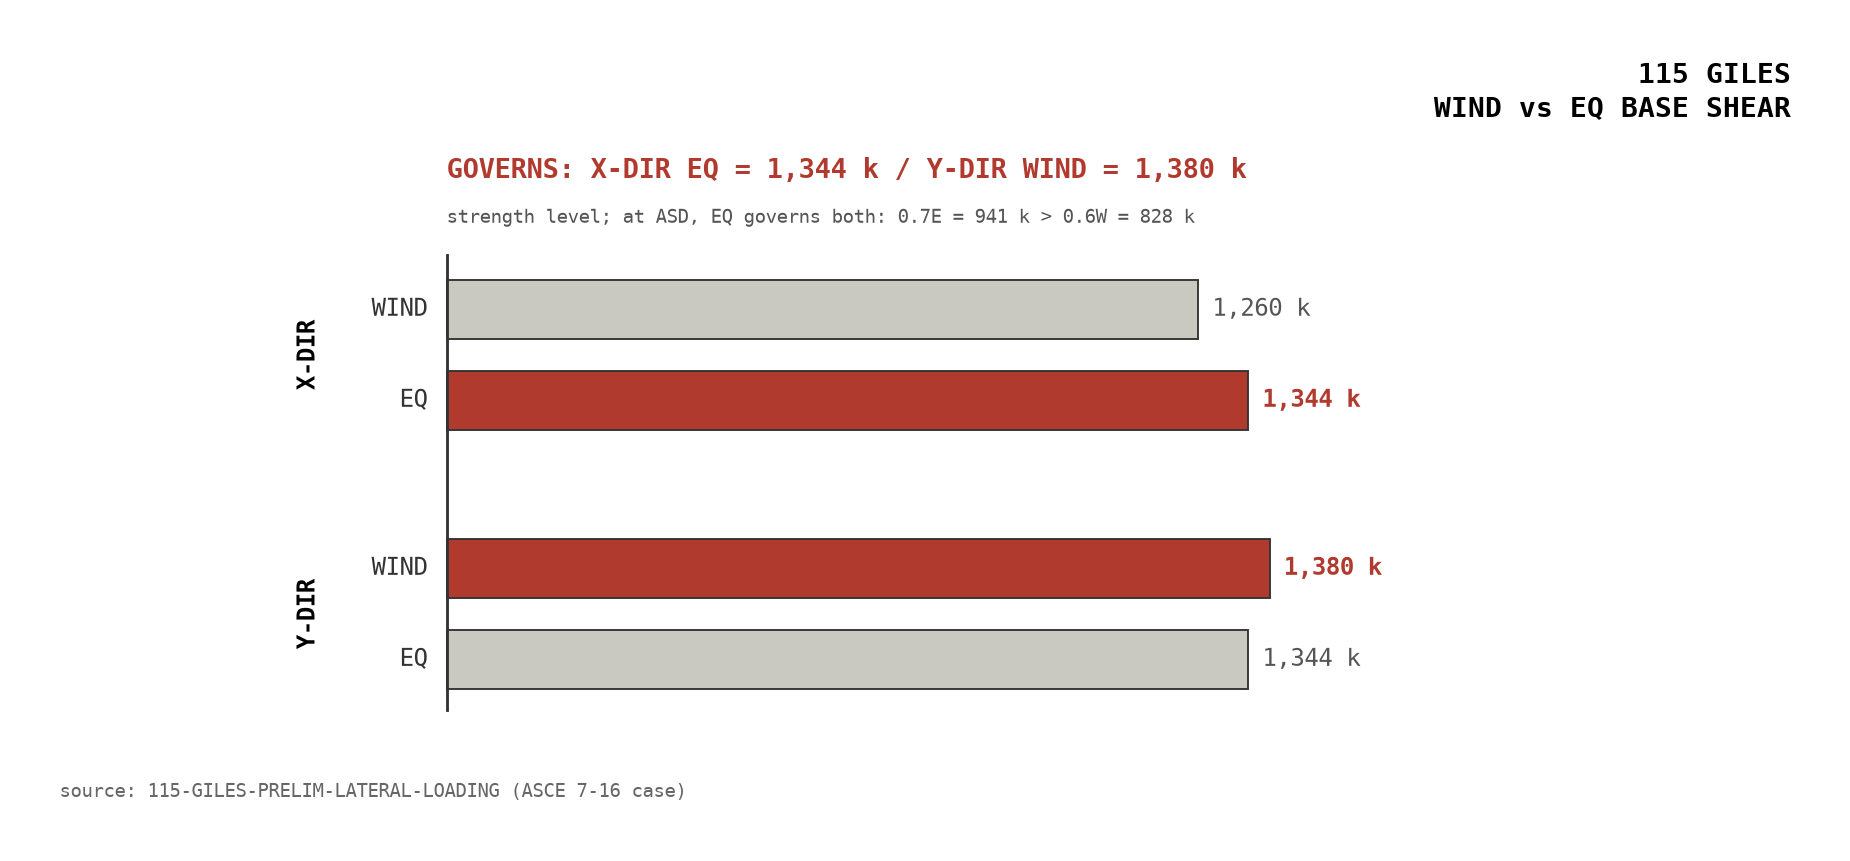
\includegraphics[width=\linewidth]{loads-summary.png}

\section{SDOF Idealization}

\noindent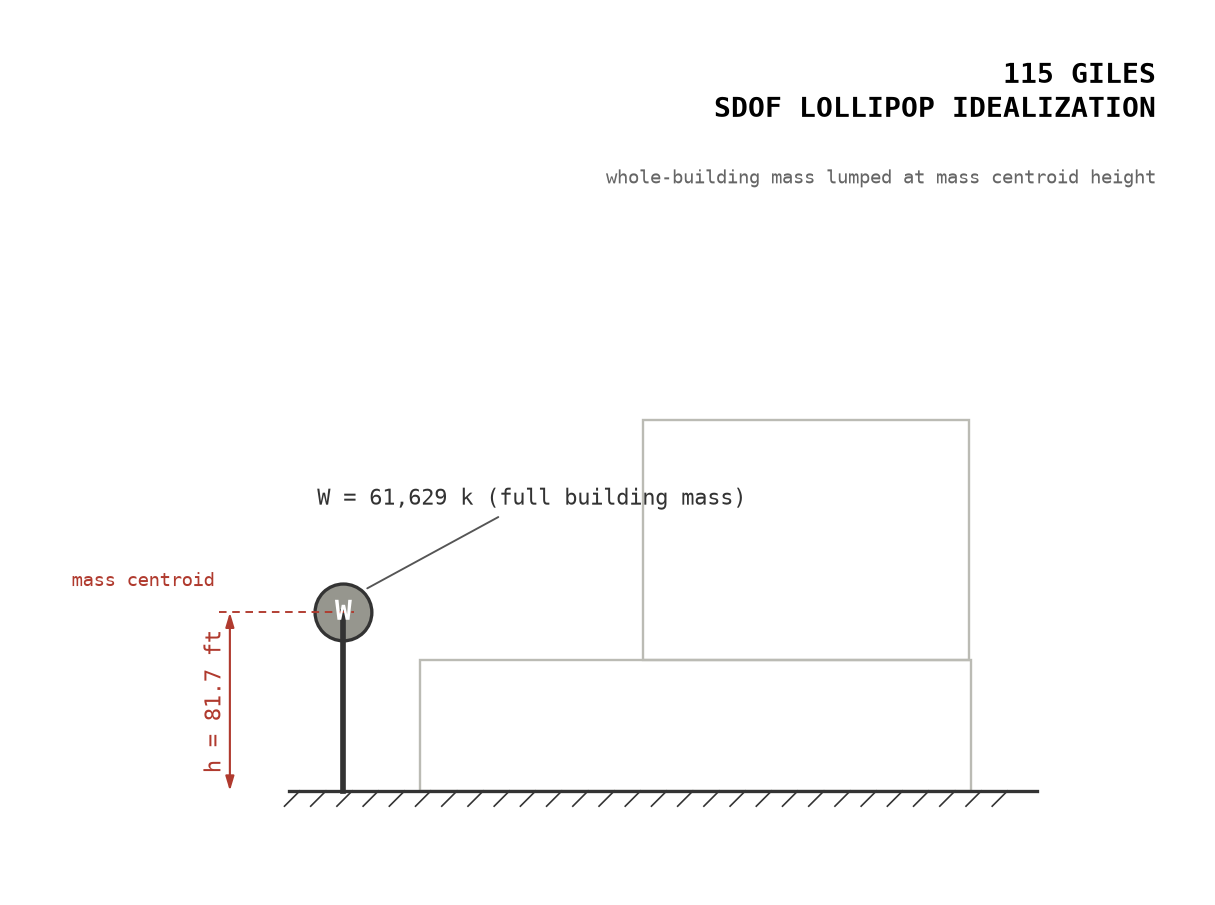
\includegraphics[width=0.85\linewidth]{lollipop.png}

\section{EQ Overturning Moment}

\noindent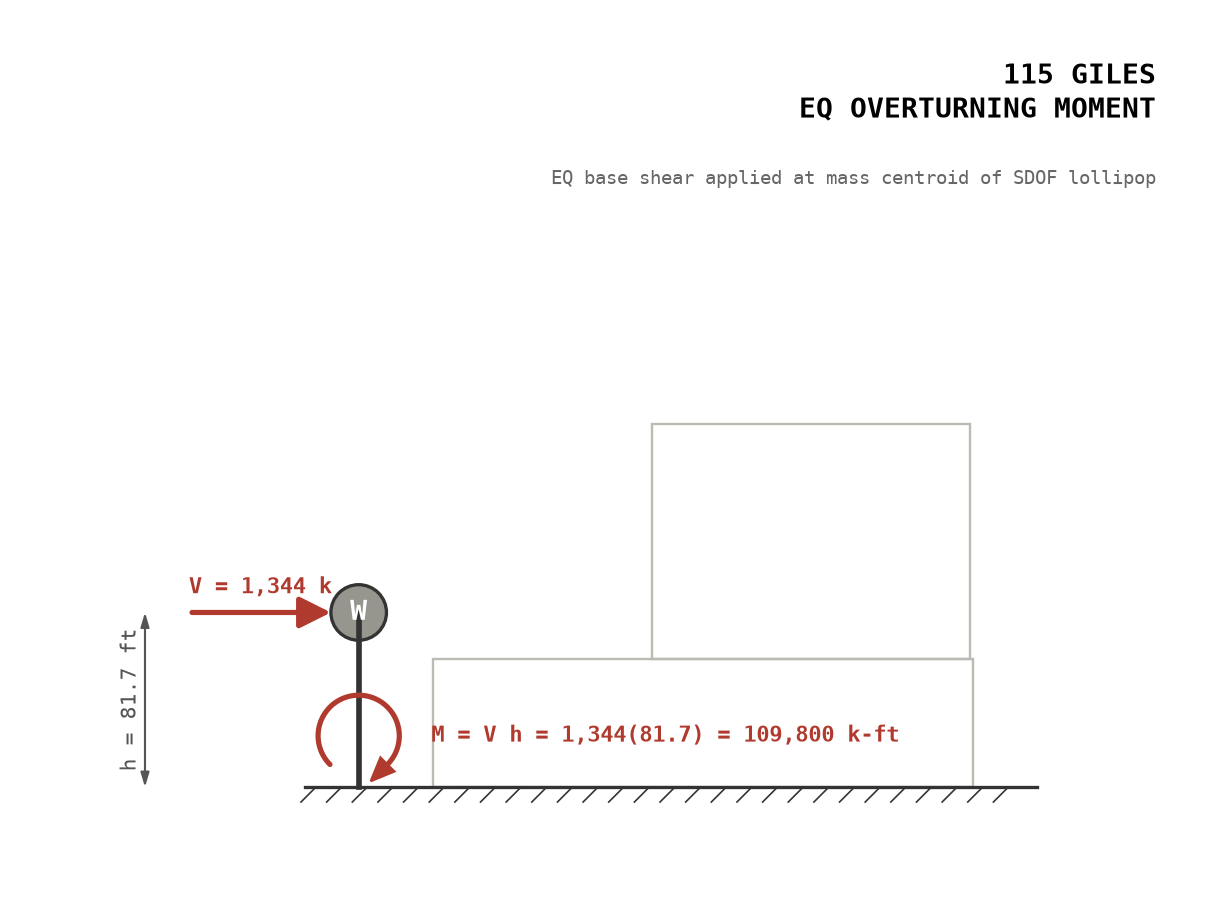
\includegraphics[width=0.85\linewidth]{overturning.png}

\newpage
\section{Wall Quantity}

5 walls at 16 ft in X, 3 walls at 16 ft in Y. Each straight wall taken separately; torsion neglected. Demand split evenly; governing case per direction (X: EQ, Y: wind, resultant at $h/2 = 85$ ft).

\begin{equation}
\text{X:} \quad V_u = \tfrac{1344}{5} = 269~\mathrm{k} \qquad M_u = \tfrac{109{,}800}{5} = 21{,}960~\mathrm{k\text{-}ft}
\end{equation}
\begin{equation}
\text{Y:} \quad V_u = \tfrac{1380}{3} = 460~\mathrm{k} \qquad M_u = \tfrac{1380(85)}{3} = 39{,}100~\mathrm{k\text{-}ft}
\end{equation}

\medskip
Section: 12 in $\times$ 16 ft, $f'_c = 5$ ksi, $f_y = 60$ ksi. Each end: 10 rows of 4\#11 at 4 in. Section and flexural capacity from concrete-beam.vercel.app:

\medskip
\noindent
\begin{minipage}[c]{0.34\linewidth}
\centering
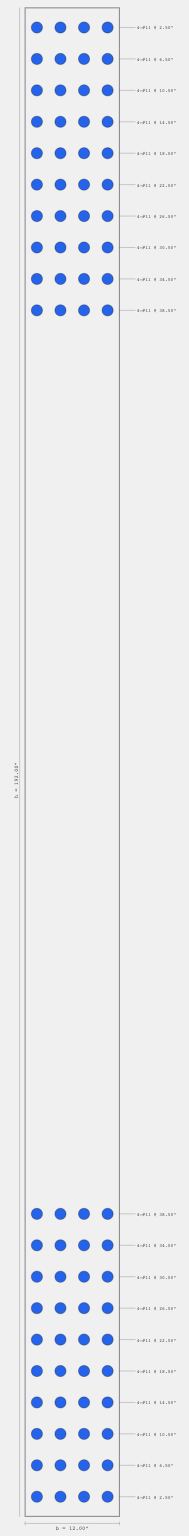
\includegraphics[height=3.1in]{wall-section-full.png}\hspace{0.4in}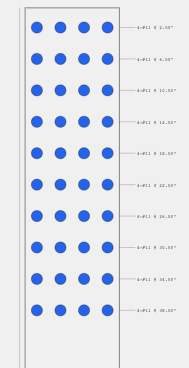
\includegraphics[height=3.1in]{wall-section-end.png}\\
{\ttfamily\footnotesize full wall \quad / \quad end zone}
\end{minipage}\hfill
\begin{minipage}[c]{0.62\linewidth}
{\ttfamily\footnotesize \begin{tabular}{@{}lr@{}}
$A_s$ (each end) & 62.46 in$^2$ \\
$d$ / $d'$ & 171.5 / 20.5 in \\
$a$ / $c$ & 28.4 / 35.5 in \\
$\varepsilon_t$ & 0.0115 (tension-controlled) \\
$\phi M_n$ & 43{,}124 k-ft \\
\end{tabular}}

\begin{equation*}
\phi V_n = \phi A_{cv}\,(2\lambda\sqrt{f'_c} + \rho_t f_y) = 0.75(2304)(141 + 150)/1000 = 504~\mathrm{k}
\end{equation*}
{\ttfamily\footnotesize \begin{tabular}{@{}ll@{}}
$\varepsilon_t$ & net tensile strain, extreme tension steel \\
$A_{cv}$ & wall shear area, $12 \times 192 = 2{,}304$ in$^2$ \\
$\rho_t$ & horizontal web reinf ratio, 0.0025 min assumed \\
\end{tabular}}

\medskip
$P = 0$ and equal end reinforcement; wall treated as vertical doubly-reinforced beam.
\end{minipage}

\medskip
{\ttfamily\footnotesize
\begin{tabular}{@{}lrr@{}}
{\scriptsize WALL} & {\scriptsize DCR V} & {\scriptsize DCR M} \\
\hline
X (5 at 16 ft) & 269/504 = 0.53 & 21{,}960/43{,}124 = 0.51 \\
Y (3 at 16 ft) & 460/504 = 0.91 & 39{,}100/43{,}124 = 0.91 \\
\end{tabular}}

\medskip
Quantity works. Y walls at DCR $\approx 0.9$ -- tight; X has margin.

\end{document}
